\chapter{Introduction}

\section{Background}

Sentence parsing is an important aspect of Natural Language Processing which is
helpful in understanding the meaning, structure, and syntactical relationships
in sentences which can further lead to more insightful tasks like knowledge
graph creation, information retrieval, question answering and machine
translation.  There are two kinds of sentence parsing:
\begin{description}
    \item [Constituency Parsing:]
        It defines the syntactical structure of a sentence by building a tree
        based on Context-Free Grammar. The words are the leaves of the tree,
        while non-leaf nodes show the abstract structure of the sentence.
        Constituency parsing is very helpful in visualizing the entire
        syntactical structure of a sentence. These parse trees can be
        useful in word processing systems for grammar checking - a
        grammatically incorrect sentence will be hard to parse. Algorithms like
        CKY(Cocke-Kasami-Younger) and shift-reduce are used for constituency
        parsing.
    \item [Dependency Parsing:]
        It defines the grammatical structure of a sentence by showing the
        dependencies among the words in the sentence. The nodes are the words
        in the sentence and the arch between the nodes are labeled by
        appropriate relation between them. A dependency parsed sentence in English looks like this:
    \begin{figure}[!h]
        \center
        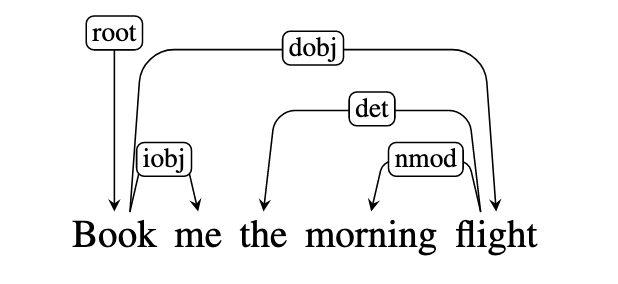
\includegraphics[scale=0.2]{images/dep_tree_eng_example}
        \caption{A dependency parsed English sentence\cite{stanfordLec}}
        \label{fig:dep_example}
    \end{figure}
    \newline
    Similarly, an example of dependency parsing in Nepali is shown below:
    \begin{figure}[!h]
        \center
        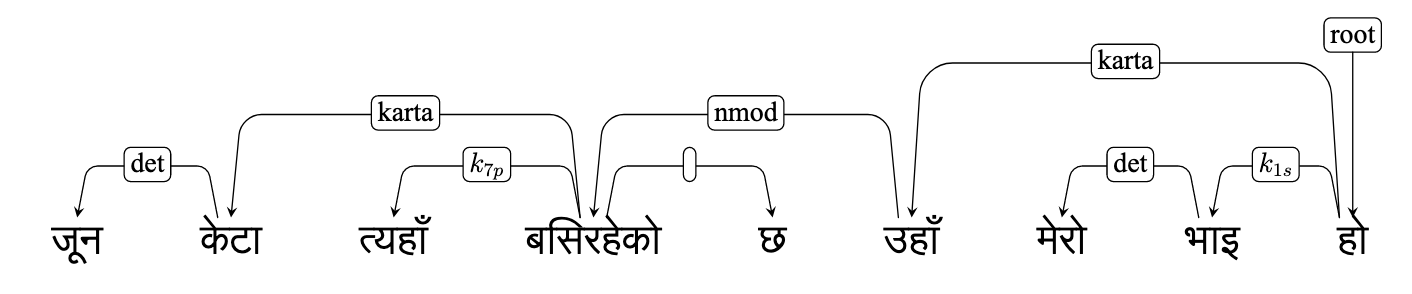
\includegraphics[scale=0.2]{images/dep_tree_example}
        \caption{A dependency parsed Nepali sentence\cite{yajnik1}}
        \label{fig:dep_example_eng}
    \end{figure}
    \newline
\end{description}
Although both kind of parsers suffer with ambiguous sentences, dependency
parser is able to handle free word order languages. However, both types of
parsing are important in computational linguistics and using one over other
generally depends on the application. In this thesis, we focus on dependency
parsing of Nepali Language.

\subsection*{Approaches to Dependency Parsing}
\subsubsection*{Transition-Based Dependency Parsing}
Transition based parsing consists of a stack on which we build the parse, a
buffer from where the input tokens to be parsed are read and a parser which
takes actions on the parse via a predictor called oracle. The parsing generally
takes place greedily.
\\~\\
The parser walks through the sentence left to right and successively shifts
items from buffer to the stack. At each step, two items from the stack are
examined and the oracle decides what action to be taken. The actions(transition
operations) are:
\begin{itemize}
    \item \textbf{LeftArc}: Assign head-dependent relation between word at the top of the stack and the second word. Remove the second word from the stack.
    \item \textbf{RightArc}: Assign head-dependent relation between second word of the stack and the top word. Remove the top word from the stack.
    \item \textbf{Shift}: Remove word from the front of the buffer and move it to the top of the stack.
\end{itemize}
The approach using these sets of operations is called \textbf{arc standard
approach} to transition-based parsing. And the major task for creating a
dependency parser is to create the oracle which is done using feature based
classifier or neural methods.
\begin{figure}[!h]
    \center
    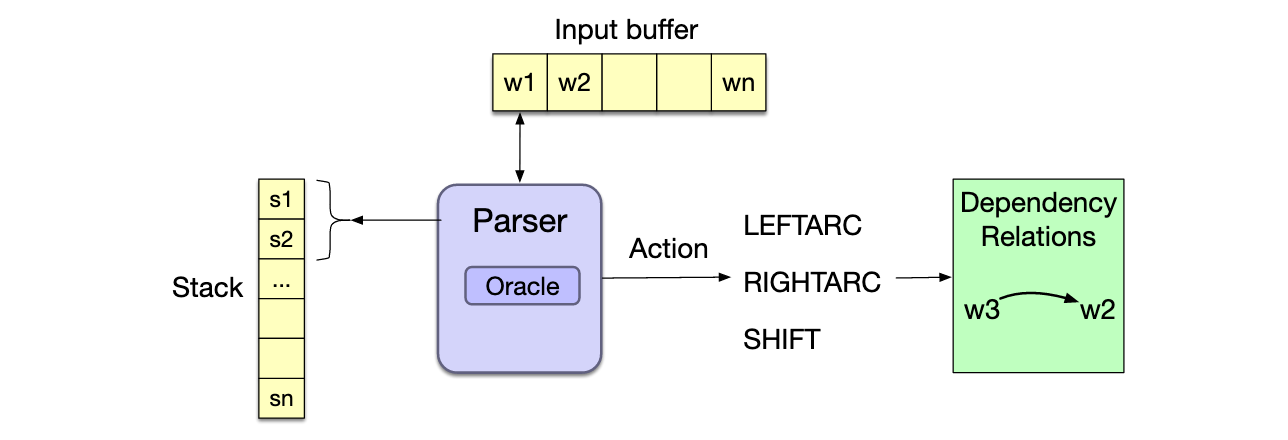
\includegraphics[scale=0.2]{images/transition_based_parser}
    \caption{Transition-based parser\cite{stanfordLec}}
    \label{fig:transition_based_parser}
\end{figure}

\subsubsection*{Graph-Based Dependency Parsing}
This is a more advanced and accurate parsing approach which shines especially
for long sentences. Transition-based methods have problems when the heads are
very far from the dependents. These are effective because rather than relying on
greedy local decisions, they score entire trees. These can also produce
non-projective parses. The general idea is to have possible trees for the
sentence, score each of them and choose the best one.
\begin{figure}[!h]
    \center
    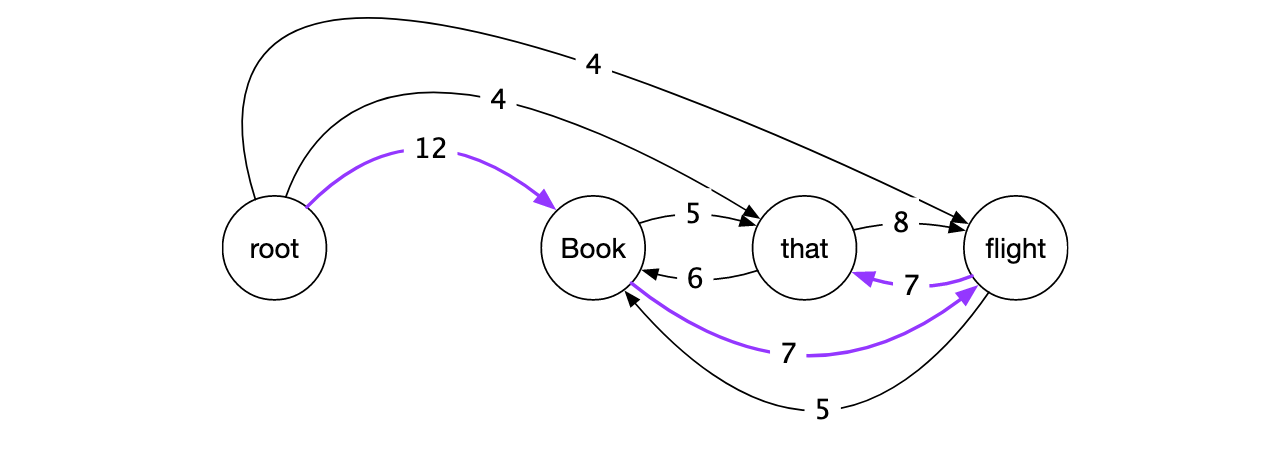
\includegraphics[scale=0.2]{images/graph-based-parser}
    \caption{Initial assignment in graph-based parsing for \textit{Book that flight}\cite{stanfordLec}}
    \label{fig:transition_based_parser}
\end{figure}

\subsection*{A Brief Note on Nepali Language}
Nepali, the national language of Nepal, is an Indo-Aryan language rooted from
Sanskrit. It is written in Devanagari script developed from  the  Brahmi
script in the 11th century AD. Nepali is spoken by about 56\% people in Nepal
which is about 16 million Nepalese. It is also spoken in other countries like
India, Bhutan and Myanmar. Despite having a considerable size of speakers,
resources suitable for computational linguistics are not readily available.
Thus, attempting to work on data intensive NLP tasks is still a challenge.
\newline
\newline
Parsing Nepali text is an interesting and challenging feat. Unlike English,
Nepali is a free order language which means the phrases in a sentences can
appear in any order. For example, consider the following two sentences:
\newline
\newline
{\dev
मैले रामलाई कलम दिएँ।
\newline
मैले कलम रामलाई दिएँ।
}
\newline
\newline
The middle two words {\dev कलम }and {\dev रामलाई} are interchanged, yet the two
sentences mean exactly the same although the first one has frequent colloquial
occurrence than the second one. Similarly, consider the following slightly
complicated sentences which have no semantic difference at all:
\newline
\newline
{\dev
मनोमानी चाँदी आयातमा राष्ट्र बैंकले लगायो रोक ।
\newline
राष्ट्र बैंकले मनोमानी चाँदी आयातमा लगायो रोक ।
\newline
मनोमानी चाँदी आयातमा राष्ट्र बैंकले रोक लगायो ।
\newline
राष्ट्र बैंकले मनोमानी चाँदी आयातमा रोक लगायो ।
}

\subsection*{BERT Model}
BERT is a transformers based bidirectional language model. The mostly used
aspects of BERT are the internal layer representations which serve as
contextual embeddings for tokens in a language. It is a state-of-the art model
upon which many improvisations and experiments have been done. In fact, BERT
represents the language tokens so well that these days, it is used for wide
varieties of downstream NLP tasks like NER, question answering and even
dependency parsing.

\subsubsection{Transformers and Attention}
Transformer is an encoder-decoder architecture which makes use of attention
mechanism unlike traditional RNN based encoding. Using attention mechanisms
avoid the two issues with RNNs: vanishing gradients and unability to
parallelize the computations. This is because RNNs are sequential whereas using
attention, all of the tokens in the sentence are taken into account at once.
Here's how \textbf{self-attention} is calculated:
\\
\begin{itemize}
    \item[1] Let initial embedding for each token be $V_i$.\\
    \item[2] For each token {i}, calculate the dot product with other tokens:
            $W_{ij} = V_i . V_j$ which is a scalar.
    \item[3] The weights $W_{ij}$ are normalized to have a sum 1.
    \item[4] Calculate the final embedding for each token as:
            $Y_i = W_{i1} V_1 + W_{i2} V_2 + W_{i3} V_3 + ... + W_{in} V_n$
    \item[5] $Y_i$s are the embeddings of the tokens based on their context.
\end{itemize}
Note that there is nothing being trained with self-attention. In order to have
better context with respect to the task at hand, the attention needs to have
some trainable parameters. The parameters are generally represented as weight
matrices.


\section {Problem Statement}
Most of the state-of-the-art dependency parsing techniques are based on
Machine Learning, especially supervised learning.  Universal Dependencies
\cite{nivreUD} treebank provides data for dependency parsing of various
languages. Unfortunately, it is still not populated with Nepali dependency
tags dataset which is the major motivation for this thesis.
\\~\\
Being a low resource language, many of the NLP applications are facing
challenges for Nepali text. Most of the works in Nepali are based on Paninian
Grammar \cite{paninianEng,yajnik1,yajnik2} which make use of
rules\cite{balCompGrammar} and formulate as Linear Programming
Problem\cite{yajnik2} or as bipartite graph\cite{yajnik1}, none of which are
data driven. Also, they do not take into account the lexical details of the
language. Although the rule-based methods themselves are robust, they suffer
from various issues like:
\begin{itemize}
    \item[1.] Not including lexical details is a huge loss of useful
        information for parsing. And including lexical information in rules is
        not feasible unless the lexicon is very small.
    \item[2.] Rule based systems are constraint based which can by their nature
        be NP-Complete and thus can result in non-termination and efficiency
        problems, for example WCDG Parser\cite{compareRuleStatistical}. As an
        example, one of the rule based systems could not even give solution to the sentence
        \dev{कार्यक्रममा विश्व बैंककी प्रबन्ध निर्देशकले खाद्य सुरक्षामा ध्यान दिन आग्रह गरेकी थिइन् ।}
    \item[3.] Chunking Rules cannot correctly parse the phrase structures, for
        example \dev{नेपाल राष्ट्र बैंक} can't be chunked correctly.
\end{itemize}
Using lexical information in rule based systems will result in an
incomprehensible rule set. Thus, the only feasible way to get around such
problems is to use deep learning approaches.

\section {Objectives}
The objectives of this thesis are:
\begin{itemize}
    \item[1.] Create a annotated dataset for Nepali language, which is a low resource language, conforming to Universal Treebank annotations.
    \item[3.] Extend the state-of-the-art parser to support multilingual learning and thus create a Nepali dependency parser.
    \item[2.] Analyze the effect of model transfer based on various source languages for parsing Nepali sentences.
\end{itemize}

\section {Scope of Applications and Contribution}
Dependency parsing basically converts unstructured text data into structured
data which can be stored in relational databases as well. It finds its
applications in various domains like:
\begin{itemize}
    \item \textbf{Natural Language Understanding}: Using numbers and embeddings
        for natural language is somehow understandable by computers but not by
        humans. Dependency parsing makes it interpretative for both humans and computers.
    \item \textbf{Sentiment Analysis}: With clearly defined components in a
        sentence, it allows aspect-oriented sentiment analysis.
    \item \textbf{Machine Translation}: Node by node translation and a sentence
        generator for parse tree can provide good-enough translations or can be
        supplement for more advanced translation systems.
    \item \textbf{Knowledge Graphs and Information Retrieval}: It also allows
        for creation of triplets for knowledge graphs which can also be
        utilized in information retrieval systems.
\end{itemize}

The main contribution of this thesis is the creation of high quality dependency
parsing annotated data. The work also presents the experimental analysis on
effect of various sizes and varieties of source languages in the
state-of-the-art multilingual model \cite{steps-parser} for Nepali Dependency
Parsing. Equally important technical contribution is the use and customization
of \cite{steps-parser} to create a dependency parsing system for Nepali
language, which had not been before. And thirdly, using the created dataset and
various other language datasets, the model is evaluated for different
configurations of source languages and dataset sizes. To our knowledge, this is
the first use of transfer learning/multilingual parsing for Nepali Language.



\section{Outline of the Thesis}
The remaining chapters are organized as follows:
\begin{itemize}
    \item \textbf{Chapter 2} describes the literature and latest advances in the field of dependency parsing.
    \item \textbf{Chapter 3} outlines the proposed methodology.
    \item \textbf{Chapter 4} outlines the results and analysis.
    \item \textbf{Chapter 5} outlines conclusions and future directions for the work.
\end{itemize}
